\chapter{Application: Interactive Semi-Structured Schema Design}
\begin{abstract}
% -*- root: ../cnf-json.tex -*-
Ad-hoc data models like \json make it easy to evolve schemas and to multiplex different data-types into a single stream.
This flexibility makes \json great for generating data, but also makes it much harder to query, ingest into a database, and index.
In this paper, we explore the first step of \json data loading: schema design.
Specifically, we consider the challenge of designing schemas for existing \json datasets as an \emph{interactive} problem.  
We present \systemnametwo, a roll-up/drill-down style interface for exploring collections of \json records.
\systemnametwo helps users to visualize the collection, identify relevant fragments, and map it down into one or more flat, relational schemas.
We describe and evaluate two key components of \systemnametwo: 
(1) A summary schema representation that significantly reduces the complexity of JSON schemas without a meaningful reduction in information content, 
and (2) A collection of schema visualizations that help users to qualitatively survey variability amongst different schemas in the collection.
\end{abstract}

\section{Introduction}
\label{sec:introduction}
% -*- root: ../cnf-json.tex -*-

Semi-structured formats like \json allow users to design schemas on-the-fly, as data is generated.
For example, adding a new attribute to the output of a system logger does not break backwards compatibility with existing data.
This flexibility facilitates the addition of new features and enables low-overhead adaptation of data-generating processes.
However, because the data does not have a consistent underlying schema, it can be harder (and slower) to explore than simple tabular data.
The logic of each and every query must explicitly account for variations in the schema like missing attributes.  
Performance also suffers, as there is no one physical data representation that is ideal for all schemas.

To address these problems, a variety of techniques~\cite{DBLP:conf/cidr/LiuG15,DBLP:conf/edbt/BaaziziLCGS17,DBLP:conf/sigmod/DiScalaA16,DBLP:conf/vldb/GoldmanW97,spoth:2017:cidr:adaptive} have arisen to generate schemas after-the-fact.
The goal of these \emph{semi-structured schema discovery} (\sssd) techniques is to propose a schema for collections of \json records.
A common approach to this problem is to bind the \json records to a normalized relational representation, or in other words, to derive a set of flat \emph{views} over the hierarchical \json data.

Existing automated approaches to this problem (e.g., \cite{DBLP:conf/sigmod/DiScalaA16,DBLP:conf/vldb/GoldmanW97}) operate in a single-pass: They propose a schema and consider their job done.
Unfortunately these techniques also rely heavily on general heuristics to select from among a set of schema design choices, as a clear declarative specification of a domain would be tantamount to having the schema already.
To supplement domain-agnostic heuristics with feedback from domain experts, we propose a new \emph{iterative and interactive} approach to \sssd called \systemnametwo.

\systemnametwo provides a OLAP-style interface (with analogs to roll-up, drill-down, and slice+dice) specialized for exploring collections of \json records.  
Every state of this interface corresponds to a relational view defined over the \json data.
When ready, this view can be exported to a classical RDBMS or similar tool for simplified, more efficient data access.
In this paper, we explore several design options for \systemnametwo, and discuss how each interacts with the challenges of \sssd.

\subsection{Extracting Relational Entities}
The first class of challenges we address involve the nuts and bolts of mapping hierarchical \json schemas to flat relational entities.  
Fundamentally, this involves a combination of three relational operators: Projection, Selection, and Unnesting.  

\tinysection{Projecting Attributes}
\json schema discovery can, naively, be thought of as a form of schema normalization~\cite{Codd:1979:EDR:320107.320109}, where each distinct path in a record is treated as its own attribute.
Entities then, are simply groups of attributes projected out of the \json data, and 
the \sssd problem reduces to finding such groups (e.g., by using Functional Dependencies~\cite{DBLP:conf/sigmod/DiScalaA16}).  

\tinysection{Selecting Records}
This naive approach fails in situations where the collection of \json records is a mix of different entity types that share properties.
As a simple example, Twitter streams mix three entity types: tweets, retweets, and deleted tweets.  
Although each entity appears in distinct records, they share attributes in common.
Hence, entity extraction is not just normalization in the classical sense of partitioning attributes, but rather also a matter of partitioning records by content.

\tinysection{Collapsing Nested Collections}
\json specifies two collection types: Arrays and Objects.  
Typically the former is used for encoding nested collections and the latter for encoding tuples with named attributes.
However, this is not a strict requirement.
For example, latitude and longitude are often encoded as a 2-element array.
Conversely, in some data sets, objects are used as way to index collections by named keys rather than by positions.
Hence, simple type analysis can not distinguish between the two cases.
This is problematic because treating a collection as a tuple creates an explosion of attributes that make classical normalization techniques incredibly expensive.

\subsection{Human-Scale \sssd}
Even in settings where \json data is comparatively well behaved, it is common for it to have dozens, or even hundreds of attributes per record.  
Similarly, individual \json records can be built from any of the hundreds or thousands (or more) different permutations of the full set of attributes used across the entire collection.
Bringing this information down to human scale requires simultaneously simplifying and summarizing.

\tinysection{Summarization}
For the purposes of entity construction, the full set of attributes is often unnecessary.
It is often possible to collapse multiple attributes together, or express attributes as equivalent alternatives.
As an example, an address might consist of four distinct attributes city, zip code, street, and number when it could conceptually be expressed as just one.

\tinysection{Visualization}
In addition to simplifying the underlying problem, it is also useful to give users a coarse ``top-down'' view of the schema process.
Specifically, users need to (1) be able to see patterns of structural similarity between distinct schemas, and (2) understand how much variation exists in the data set as-is.

\tinysection{Iteration}
By combining straightforward summarization and data visualization techniques, \systemnametwo helps users to quickly identify natural clusters of records and attributes that represent relational entities.
\systemnametwo facilitates an \emph{iterative} schema design process to allow human experts to better evaluate whether structures in the data indicate conceptual relationships between records or attributes, or are merely data artifacts.

\begin{figure}
\centering
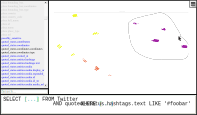
\includegraphics[width=0.9\linewidth]{SchemaSummarization/img/UI}
\caption{Prototype user interface for \systemnametwo.}
\label{fig:ui}
\end{figure}

\subsection{Overview}
Figure~\ref{fig:ui} shows the prototype interface of \systemnametwo. 
The pane on the left, discussed in Section~\ref{sec:distribution}, shows the schema of the currently selected JSON view, highlighting attributes and groups based on relevance.
The pane on the right, discussed in Section~\ref{sec:visualization}, provides a top-down visual sketch of schemas in the currently selected JSON data, and allows users to interactively filter out parts of it.
Finally in Section~\ref{sec:visualization}, we show examples of how \systemnametwo facilitates incremental, iterative exploration and mapping of JSON schemas.






\section{Summarization}
\label{sec:distribution}
% !TEX root = ../cnf-json.tex
The first component of \systemnametwo, the schema pane, shows the relational schema of the extracted view.
Initially, this schema consists of one attribute for every path in the \json collection being summarized.
Attributes may be deleted or restored, and sets of attributes may be unified.

The core challenge behind implementing this pane is that, depending on data set, the schema could consist of hundreds or thousands of attributes.
This can be overwhelming for users who just wants to find account profiles appearing in a Twitter stream.
To mitigate this problem, \systemnametwo presents the schema in a summarized form.

Specifically, attributes are grouped based on both correlations and anti-correlations between them.
Groups of \emph{correlated} attributes, or those that frequently co-occur in \json records are likely to be part of a common structure.
Similarly, groups of \emph{anti-correlated} attributes, or those that rarely co-occur in \json records are likely to represent alternatives (e.g., a Street Address vs GPS coordinates).  
We use correlations and anti-correlations between attributes to compact the schema for representation.
Before describing the summary itself, we first formalize the problem.

%%%%%%%%%%%%%%%%%%%%%%%%%%%%%%%%%%%%%%%%%%%%%%%%%%%%%%%%%%%%%%%%%%%%

\subsection{Data Model}
A \json object is an order-independent mapping from keys to values.
A key is a unique identifier of a \json object, typically a string.
A value may be atomic or complex. 
Atomic values in \json may be integers, reals, strings, or booleans.
A complex value is either a nested object, or an \textit{array}, an indexed list of values.  
For simplicity, we model arrays as objects by treating array indexes as keys.
A \json record may be any value type, but for simplicity of exposition we will assume that all records are objects.  
\begin{example}
\label{example:jsonobject}
A fragment of Twitter Tweet encoded as \json
\begin{lstlisting}[language=json]
"tweet": {
  "text": "#SIGMOD2018 in Houston this year",
  "user": { 
    "name" : "Alice Smith",  "id" : 12345, 
    "friends_count": 1023,  …
  },
  "retweeted_status": {
    "tweet": {
      "user": { … }, "entities": { … }, 
      "place": { … }, "extended_entities": { … }
    }, …
  },
  "place": { … }, "extended_entities": { … },  
  "entities": { "hashtags": [ "SIGMOD2018" ], … },
  …
}
\end{lstlisting}
\end{example}

\noindent 
\json objects are typically viewed as trees with atomic values at the leaves, complex values as inner nodes, and edges labeled with the keys of each child.
Our goal is to identify commonalities in the structure of this tree across multiple \json records in a collection.  
To capture the structure, we define the \textit{schema} $S$ of a \json record as the record with all leaf values replaced by a constant $\bot$.
A \emph{path} $P$ is a sequence of keys $P = (k_0, \ldots, k_N)$.
For convenience, we will write paths using dots to separate keys (e.g., \inlinejson{tweet.text}).
We say that a path appears in a schema (denoted $P \in S$) if it is possible to start at the root of $S$ and traverse edges in order. 
If the value reached by this traversal is $\bot$, we say that $P$ is a terminal path of $S$ (denoted $P \bot S$).

\subsection{Paths as Attributes}
Ultimately, our goal is to create a flat, relational representation suitable for use with an entire collection of \json records.
The first step to reaching this goal is to flatten individual \json schemas into collections of attributes.
We begin with a naive translation where each attribute corresponds to one terminal path in the schema.
We write $S^\bot$ to denote the path set, or relational schema of \json schema $S$, defined as:
$
S^\bot = \comprehension{P}{P \bot S}
$
Since keys are unique, commutative and associative, this representation is interchangeable\footnote{modulo empty objects or arrays} with the tree representation.
Hence, when clear from context we will abuse syntax, using $S$ to denote both a schema and its path set.
% Hence, without loss of generality, from this point on we refer to terminal path sets as just schemas.
\begin{example}
The path set of the \json object from Example~\ref{example:jsonobject} includes the paths:
\begin{enumerate*}
  \item \inlinejson{tweet.text} \;
  \item \inlinejson{tweet.user.friends\_count}
  \item \inlinejson{tweet.user.id}\;
  \item \inlinejson{tweet.entities.hashtags.[0]}
\end{enumerate*}
Each terminal appears in the set.  Note in particular that single element of the array at \inlinejson{tweet.entities.hashtags} is assigned the key \inlinejson{[0]}.
\end{example}
Path sets make it possible to consider containment relationships between schemas.  
We say that $S_1$ is contained in $S_2$ iff $S_1^\bot \subseteq S_2^\bot$.

%%%%%%%%%%%%%%%%%%%%%%%%%%%%%%%%%%%%%%%%%%%%%%%%%%%%%%%%%%%%%%%%%%%%

\subsection{Schema Collections}
We now return to our main goal, summarizing the schemas of collections of \json records.  
The starting point for this process is the schemas themselves.  
Given a collection of \json records, we can extract the set of schemas $\{\;S_1, \ldots, S_N\;\}$ of records in the collection, which we call the \emph{source schemas}.
One existing technique for summarizing these records, used by Oracle's JSON Data Guides~\cite{oracledataguide,DBLP:conf/sigmod/LiuHMLC16}, is to simply present the set of all paths that appear anywhere in this collection.
We call this the \emph{joint schema} $\mathbb S$:
$$\mathbb S^\bot \;\;\; \defineeq \;\;\; \bigcup_i S_i^\bot$$
Observe that, by definition, each of the source schemas is contained in the joint schema.
The joint schema mirrors existing schemes for relational access to JSON data like  for example.  
However, the joint schema can still be very large, with hundreds, thousands, or even tens of thousands of columns\footnote{One dataset~\cite{pharmadata} achieved 2.4~thousand paths through nested collections of objects.}.
To summarize them we need an even more compact encoding for sets of schemas.  

\tinysection{A Schema Algebra}
As a basis for compacting schema sets, we define a simple algebra.
Recall that we are particularly interested in summarizing cooccurrence and anti-cooccurence relationships between attributes.
$$\mathbf{A}\;\;:=\;\;\mathbf{P}\;\;|\;\;\emptyset\;\;|\;\;\mathbf{A} \wedge \mathbf{A}\;\;|\;\;\mathbf{A} \vee \mathbf{A}$$
Expressions in the algebra construct sets of schemas from individual attributes.
There are two types of leaf expressions in the algebra:
A single terminal path $P$ represents a singleton schema ($\big\{\{P\}\big\}$), while $\emptyset$ denotes a set containing no schemas $\big\{\big\}$.
Disjunction acts as union, merging its two input sets:
$$
\{\;S_1, \ldots, S_N\;\} \vee \{\;S'_1, \ldots, S'_M\;\} 
\defineeq
\{\;S_1, \ldots, S_N, S'_1, \ldots, S'_M\;\}
$$
Disjunction models anti-correlation: The resulting schema set is effectively a collection of schema alternatives.  
For example, $P_1 \vee P_2$ indicates two alternative schemas: $\{P_1\}$ or $\{P_2\}$.
Conjunction combines schema sets by cartesian product:
{\small
$$
\{\;S_1, \ldots, S_N\;\} \wedge \{\;S'_1, \ldots, S'_M\;\} 
\defineeq 
\comprehension{ S_i \cup S'_j}{ i \in [1,N], j \in [1, M] }
$$
}
Conjunction models correlations: The resulting schema set mandates that exactly one option from the left-hand-side and one option from the right-hand-side be present.
On singleton inputs, the result is also a singleton.
For example, $P_1 \wedge P_2$ is a single schema that includes both $P_1$ and $P_2$.  
For inputs larger than one element, the conjunction requires one choice from each input.
For example, $(P_1\vee P_2)\wedge(P_3 \vee P_4)$ is the set of all schemas consisting of one of $P_1$ or $P_2$, and also one of $P_3$ or $P_4$.

Although we omit the proofs for conciseness, both $\wedge$ and $\vee$ are commutative and associative, and $\vee$ distributes over $\wedge$\footnote{To be precise, the structure $\tuple{\big\{\{\mathbf P\}\big\}, \vee, \wedge, \emptyset, \big\{\{\}\big\}}$ is a semiring.}.
For conciseness, we use the following syntactic conventions:
(1)~When clear from context, a schema $S$ denotes its own singleton set, and (2)~We write $P_1P_2$ to denote $P_1 \wedge P_2$.

This schema algebra gives us a range of ways to represent schema sets.
At one extreme, the set of source schemas arrives in what is effectively disjunctive normal form (DNF).
One schema may be expressed as a conjunction of its elements, and the full set of source schemas can be constructed by disjunction.
For example, the source schemas $\{P_1, P_2\}$ and $\{P_2, P_3\}$ may be represented in the algebra as $P_1P_2 \vee P_2P_3$.

At the other extreme, the joint schema is a superset of all of the source schemas.
It too can be thought of as a schema set, albeit one that loses information about which attributes appear in which schemas.
Hence, this joint schema set may be defined as the power set of all attributes in the joint schema.
$$2^{\mathbb S} = \bigwedge_{P \in \mathbb S} (P \vee \emptyset)$$
Observe that at a minimum, each of the source schemas must appear in this schema set ($S_i \in 2^{\mathbb S}$).
However many other schemas appear in the resulting schema set as well.

% We start from the original representation of the schema distribution.
% Continuing Example~\ref{example:Log}, each schema in the example can be interpreted as a \textit{conjunction} over its set of attributes, e.g. $\vec v_1= (x_1\land x_2\land \neg x_3)$.
% Uniformly drawn from the log, a schema $\vec v$ can either be $\vec v_1$, $\vec v_2$ or $\vec v_3$.
% Namely the log is essentially a \textit{disjunction} over its schema $L= (\vec v_1\lor \vec v_2 \lor \vec v_3)$.
% We will then show that there is an general algebraic structure (i.e, commutative semiring) that can describe all schema distributions.
% To represent absence of some attributes in a more compact way other than listing their negation, we define a distinguished element $1$ or empty attribute $\emptyset$ such that $\vec v \land \emptyset=\vec v$. 
% In most cases, the distinguished element $1$ is omitted. 
% For example, $\vec v_1=(x_1\land x_2)$ which implies that all other attributes \textit{except for} $x_1,x_2$ exist in the schema. 
% In addition, to merge two logs where one is empty, we define a distinguished element $0$ or empty attribute set $\{\}$ such that  $\vec v \lor \{\}= \vec v$.
% The logs of \json schema can thus be interpreted as a polynomial with respect to the semiring $\tuple{A,\land,\lor,\{\},\emptyset}$ over the space of attributes $A$.

% \tinysection{Factorization}
% The original polynomial representation can be too verbose. 
% Notice that attribute $x_1=1$ is shared by all schemas in Example~\ref{example:Log}.
% We can thus \textit{factorize} the polynomial into
% $$
% L =x_1\land (x_2\lor x_2\lor x_3)
% $$
% Note $x_2$ is duplicated in disjunction.
% We can further reduce the verbosity by introducing frequencies
% $$
% L = x_1\cdot (\frac{2}{3}\cdot x_2+ \frac{1}{3}\cdot x_3)
% $$
% Note that we replace $\land,\lor$ with $\cdot,+$ for notation consistency.
% By using above representation, the schema distribution $p(V\;|\;L)$ for Example~\ref{example:Log} can be compactly interpreted as "$x_1$ always exists while $x_2, x_3$ alternatively co-exist with $x_1$ with probability $\frac{2}{3}, \frac{1}{3}$ respectively".

% \tinysection{Polynomial Modification}
% In cases where even the optimal factorization is still too verbose, we may want to edit the polynomial, delete or insert some terms.
% For example, consider the polynomial $f_0\cdot (\frac{1}{n}\cdot f_1+\ldots +\frac{1}{n}\cdot f_n)$ where $n$ is considerably large.
% It shows that each $f_i, i=1,\ldots,n$ does not co-exist with $f_0$ very often and in some cases it is tolerable to simply ignore them.
% In other words, we modify each term in the polynomial and delete features other than $f_0$.
% This leads to a lossy representation and we will discuss how to measure the degree of information loss in Section~\ref{}\todo{}.

% \tinysection{Pattern-based Summary}
% In most cases, we seek for a compact representation that preserves frequently shared \textit{patterns} as much as possible.
% More formally, we define a pattern as any set of features $\vec v'$ (i.e., partial schema) that may be contained in some schema $\vec v$ in the log.

% \tinysection{Summary Verbosity}

% \tinysection{Definition of Information Loss}


%%%%%%%%%%%%%%%%%%%%%%%%%%%%%%%%%%%%%%%%%%%%%%%%%%%%%%%%%%%%%%%%%%%%

\subsection{Summarizing Schema Collections}
These two extreme representations (the raw source schemas and the joint schema set) are bad, but for subtly different reasons.
In both cases, the representation is too verbose.
In the former case verboseness stems from redundancy, with significant overlap in variables between the source schemas.
Conversely in the latter case it stems from imprecision, as the schema set encompasses schemas that do not appear in the source schemas.
Of the two, the latter is more compact, in particular because each attribute appears no more than once.
This is a distinct representational advantage because the joint schema can be displayed simply as a list.

We would like to preserve this only-once property.
Our aim then, is to derive an algebraic expression (1) in which each attribute appears exactly once, and (2) that is as tight a fit to the original source schema set as possible.
Ultimately, this problem reduces to polynomial factorization and the discovery of read-once formulas~\cite{Dalvi:2013:DPI:2395116.2395119}, a problem that is, in general, worse than P-time~\cite{DBLP:conf/focs/Burgisser01}.
Hence, for this paper, approximations are required.
We consider two approaches and allow the user to select the most appropriate one for their needs.
The first is based on Frequent Pattern Trees~\cite{DBLP:conf/sigmod/HanPY00} (FPTrees), a data structure commonly used for frequent pattern mining.
The second is to limit our search to read-once conjunctions of disjunctions of conjunctions, a form we call RCDC.

\begin{figure}
\centering
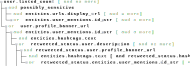
\includegraphics[width=\columnwidth]{SchemaSummarization/img/collapse-FPTree}
\caption{FP-Tree based schema summaries}
\label{fig:summary:fptree}
\end{figure}

\tinysection{FP-Tree Summaries}
An FP-Tree is a trie-like data structure that makes it easier to identify common patterns in a query.  
Every edge in the tree represents the inclusion of one feature, or in our case one attribute.
Hence, every node in the tree corresponds to a set of paths (obtained by traversal from the root), and every leaf corresponds to one source schema.
We observe that every node in an FP tree corresponds to a disjunction: For a node with 3 children, each subtree represents a different branch.  
Similarly, every edge corresponds to a conjunction with a singleton.
Although the resulting tree may duplicate some attributes, duplications are minimized~\cite{DBLP:conf/sigmod/HanPY00}.

\begin{example}
Figure~\ref{fig:summary:fptree} illustrates a schema summary based on  FP-Trees.  
Sequences of nodes with a single child are collapsed into single rows of the display (e.g., \inlinejson{user.listed_count} and 63 immediate descendents).
A toggle switch allows these entities to be displayed to the user, if desired.
Every level of the tree represents a set of alternatives. For example, \inlinejson{possibly_sensitive} never co-occurs with \inlinejson{user.profile_banner_url}.  
\end{example}

\tinysection{RCDC Summaries}
Our second visualization is based on correlations and anticorrelations.
To construct this visualization, we begin with the joint summary.
Recall that the joint summary has the form 
$$(P_1 \vee \emptyset)\;(P_2 \vee \emptyset)\;(P_3 \vee \emptyset)\;(P_4 \vee \emptyset)\ldots$$

We create a covariance matrix based on the probability of two attributes co-occurring in the schemas of one of our input \json records.  
Using this covariance matrix, hierarchical clustering~\cite{Johnson1967}, and a user-controlled threshold on the covariance, we cluster the attributes by parenthesizing.  For example, clustering might group $P_1$ with $P_2$ and likewise $P_3$ with $P_4$.
We can rewrite this formula as:
$$\approx (P_1P_2 \vee \emptyset)\;(P_3P_4 \vee \emptyset)\ldots$$
Observe that this formula omits schemas that the original formula captures (e.g., any schema including $P_1$ but not $P_2$).
However, because clustering ensures that attributes within a group co-occur frequently, there are comparatively few such schemas.

We next repeat the process with a new covariance matrix built using the frequency of co-occurrence of \emph{groups} (like $P_1P_2$).  
As before, we create clusters, but this time we cluster based on extremely negative co-variances.
Hence, members of the resulting clusters are unlikely to co-occur.
Continuing the example, let us assume that $P_1P_2$ and $P_3P_4$ are highly anti-correlated.  
Approximating and simplifying, we get an expression in RCDC form.
$$\approx (P_1P_2 \vee P_3P_4 \vee \emptyset)\ldots$$
As with the FP-Tree display, we use counts and an example attribute as a summary name for the group, and a toggle button to allow users to expand the group along either the OR or AND axes.

\begin{figure}
\centering
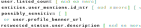
\includegraphics[width=0.8\columnwidth]{SchemaSummarization/img/collapse-RCDC}
\caption{RCDC based schema summaries}
\label{fig:summary:rcdc}
\end{figure}






\section{Visualization}
\label{sec:visualization}
% !TEX root = ../cnf-json.tex

Even within a mostly standardized collection of records like exported Twitter or Yelp data or production system logs, it is possible to find a range of schema usage patterns.
Grouping by [anti-]cooccurrence is one step towards helping users understand these usage patterns, but is insufficient for three reasons:
\begin{enumerate*}
  \item Conceptually distinct fragments of the schema may share attributes in common (e.g., delete tweet records share attributes in common with tweet records).
  \item Even if they do not co-occur, certain [groups of] attributes may be correlated (e.g., due to mobile phones, tweets with photos are also often geotagged).
  \item There is no general way to differentiate \json objects and arrays being used to represent collections from those being used to represent structures (e.g., twitter stores geographical coordinates as a 2-element array).
\end{enumerate*}
The second part of the \systemnametwo interface addresses these issues by presenting top-down visual surveys of the schema.
These surveys help users to quickly assess variations in schema usage across the collection, to identify related schema structures, and to ``drill down'' into finer grained relationships.

%Imagine an analyst is given a mixture of these Twitter \json objects and have two tasks, one where they need to use attributes of user based on tweets, and another where they need to determine 

%\begin{itemize}
%\item user will want to start with one \json schema and want to end with multiple views for different use cases
%\item Problem statement: \json schemas are often 'wide' and contain different sub schemas that map to potential use cases
%\item Through different means we try and recover these use cases and segment the data on these features
%\item then try and prompt the user to generate views until they have all their use cases met
%\end{itemize}

\begin{figure}
  \centering
  \begin{subfigure}{0.4\columnwidth}
    \centering
    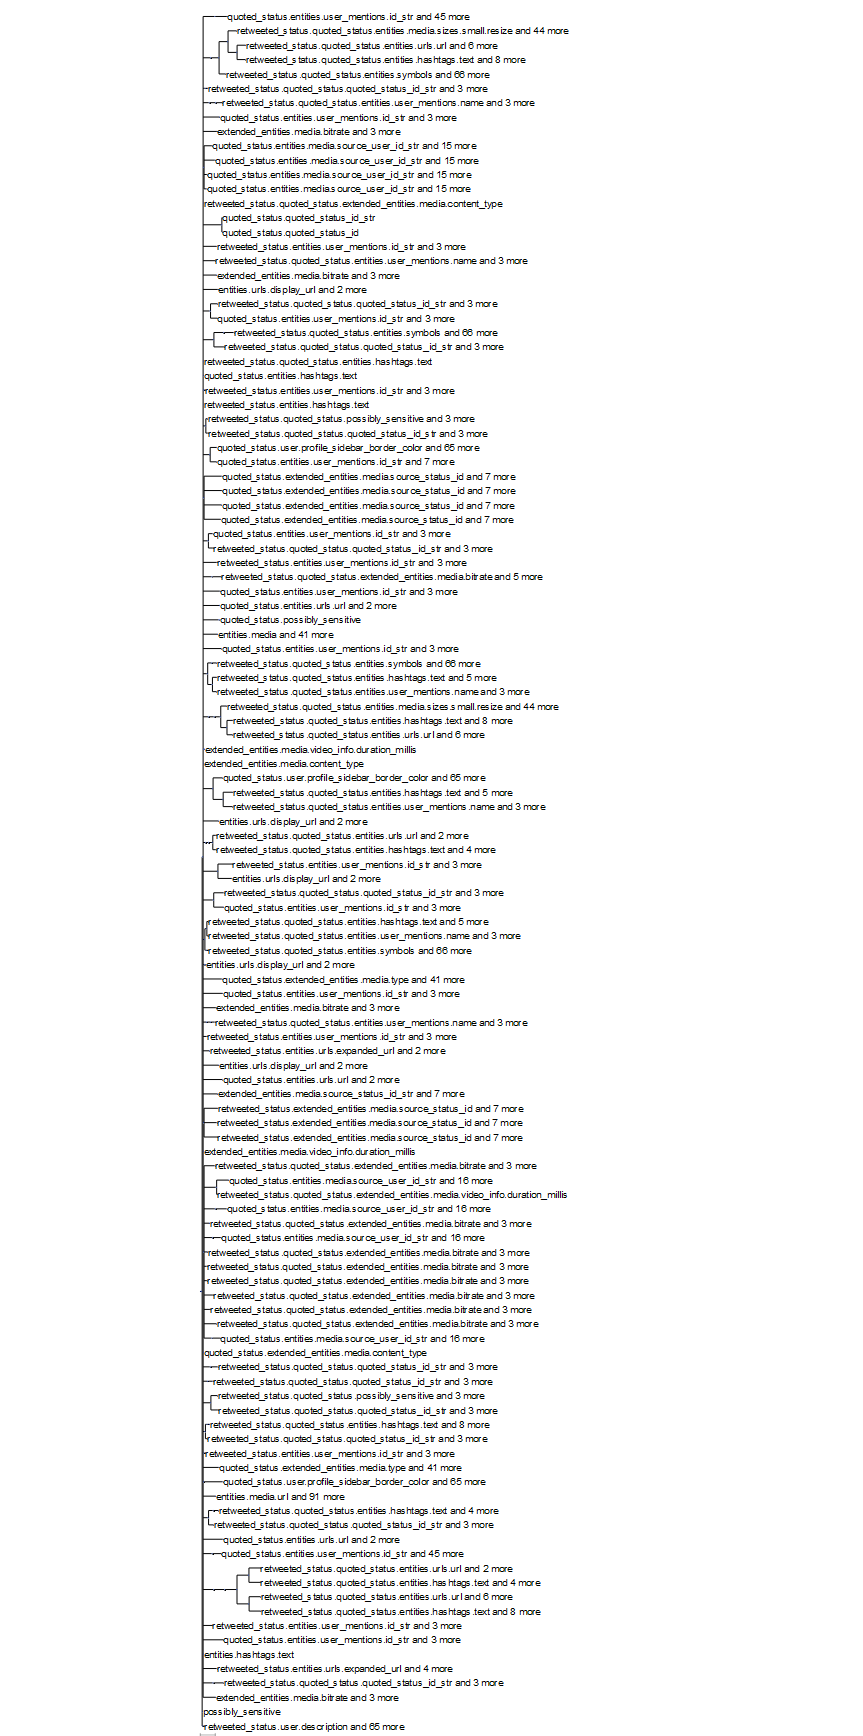
\includegraphics[width=0.57\textwidth]{SchemaSummarization/img/twitterFullTree.png}
    \caption{Without segmentation.}
    \label{fig:seg:twitterFull}
  \end{subfigure}
  \begin{subfigure}{0.59\columnwidth}
    \centering
    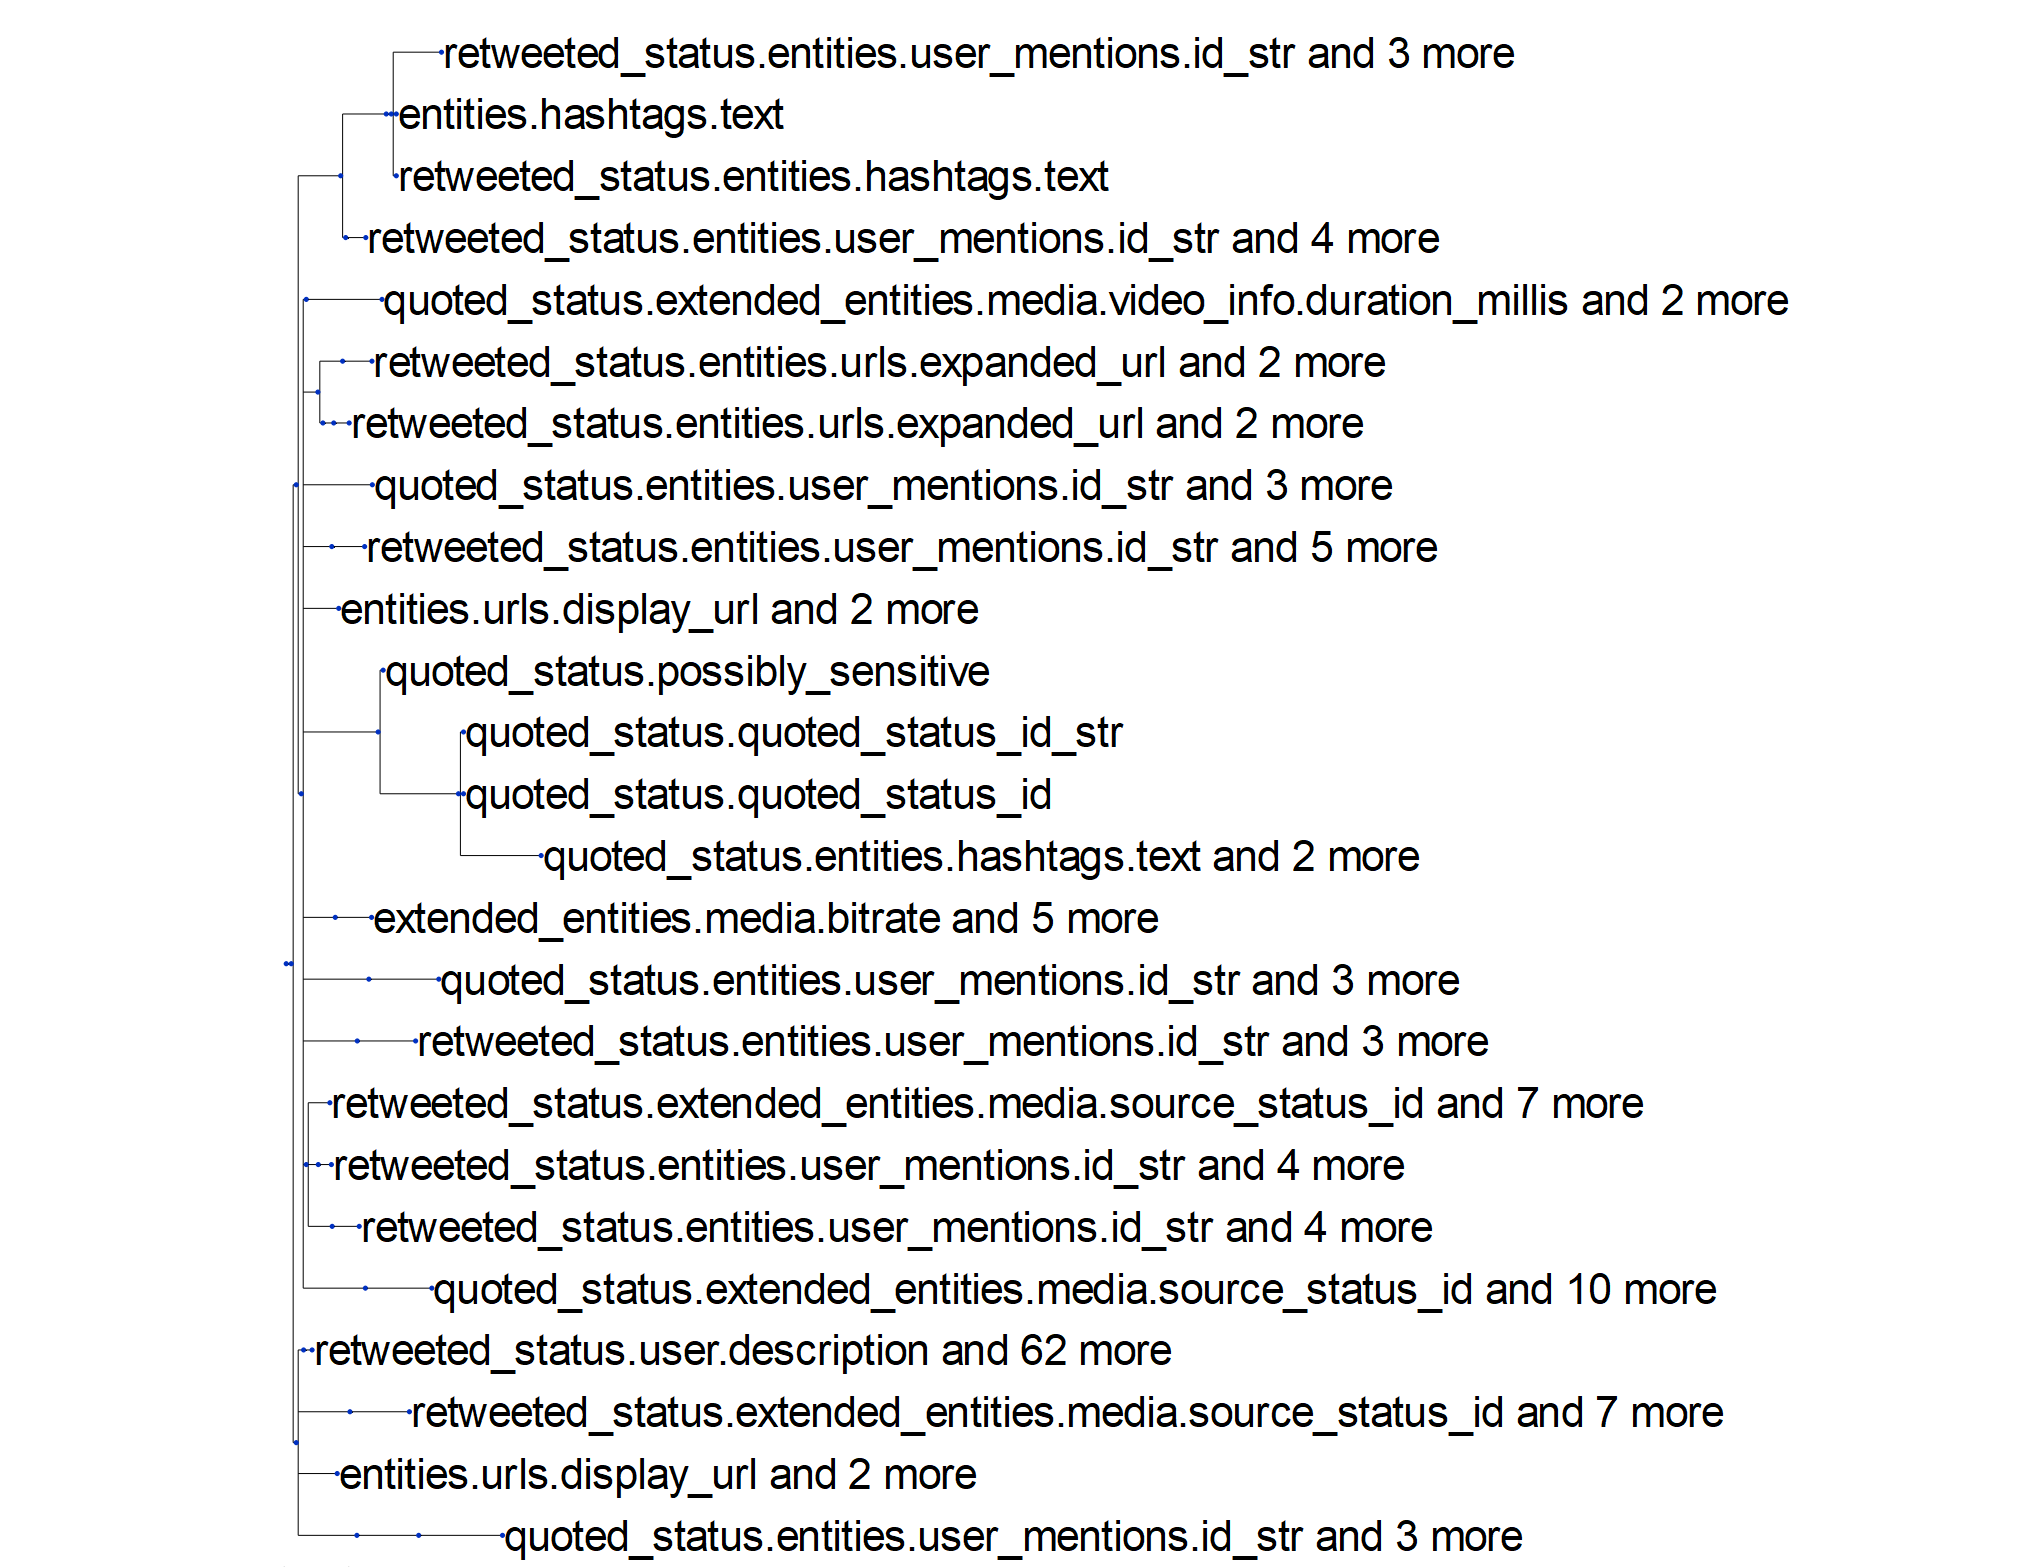
\includegraphics[width=\textwidth]{SchemaSummarization/img/twitterSegment.png}
    \caption{With segmentation.}
    \label{fig:seg:twitterSeg}
  \end{subfigure}
  \caption{Segmentation breaks up schema representations into manageable chunks.}
  \label{fig:seg}
\end{figure}

\subsection{Schema Segmentation}
Specifically, we want to help the user to focus on particular parts of the joint schema;
We want to allow the user to filter out, or segment the schema based on certain required attributes that we call \emph{subschemas}.
We define a subschema $s$ as a set of attributes, where $s$ is contained in one or more source schemas.
Further, the $s$-segment of source schemas $S_1, \ldots, S_N$ to be the subset that contain $s$:
$$\textbf{segment}(s) \defineeq \comprehension{S_i}{i \in [1,N] \wedge s \subseteq S_i}$$
We are specifically interested in visual representations that can help users to identify subschemas of interest.
By then focusing solely on the segments defined by these subschemas can significantly reduce the complexity of the schema design problem, as illustrated in Figure~\ref{fig:seg}.
Figures~\ref{fig:seg:twitterFull} illustrates the full schema summary as a tree, while Figure~\ref{fig:seg:twitterSeg} shows a partial summary identified by the user using the lasso tool we describe shortly.

\begin{figure}[H]
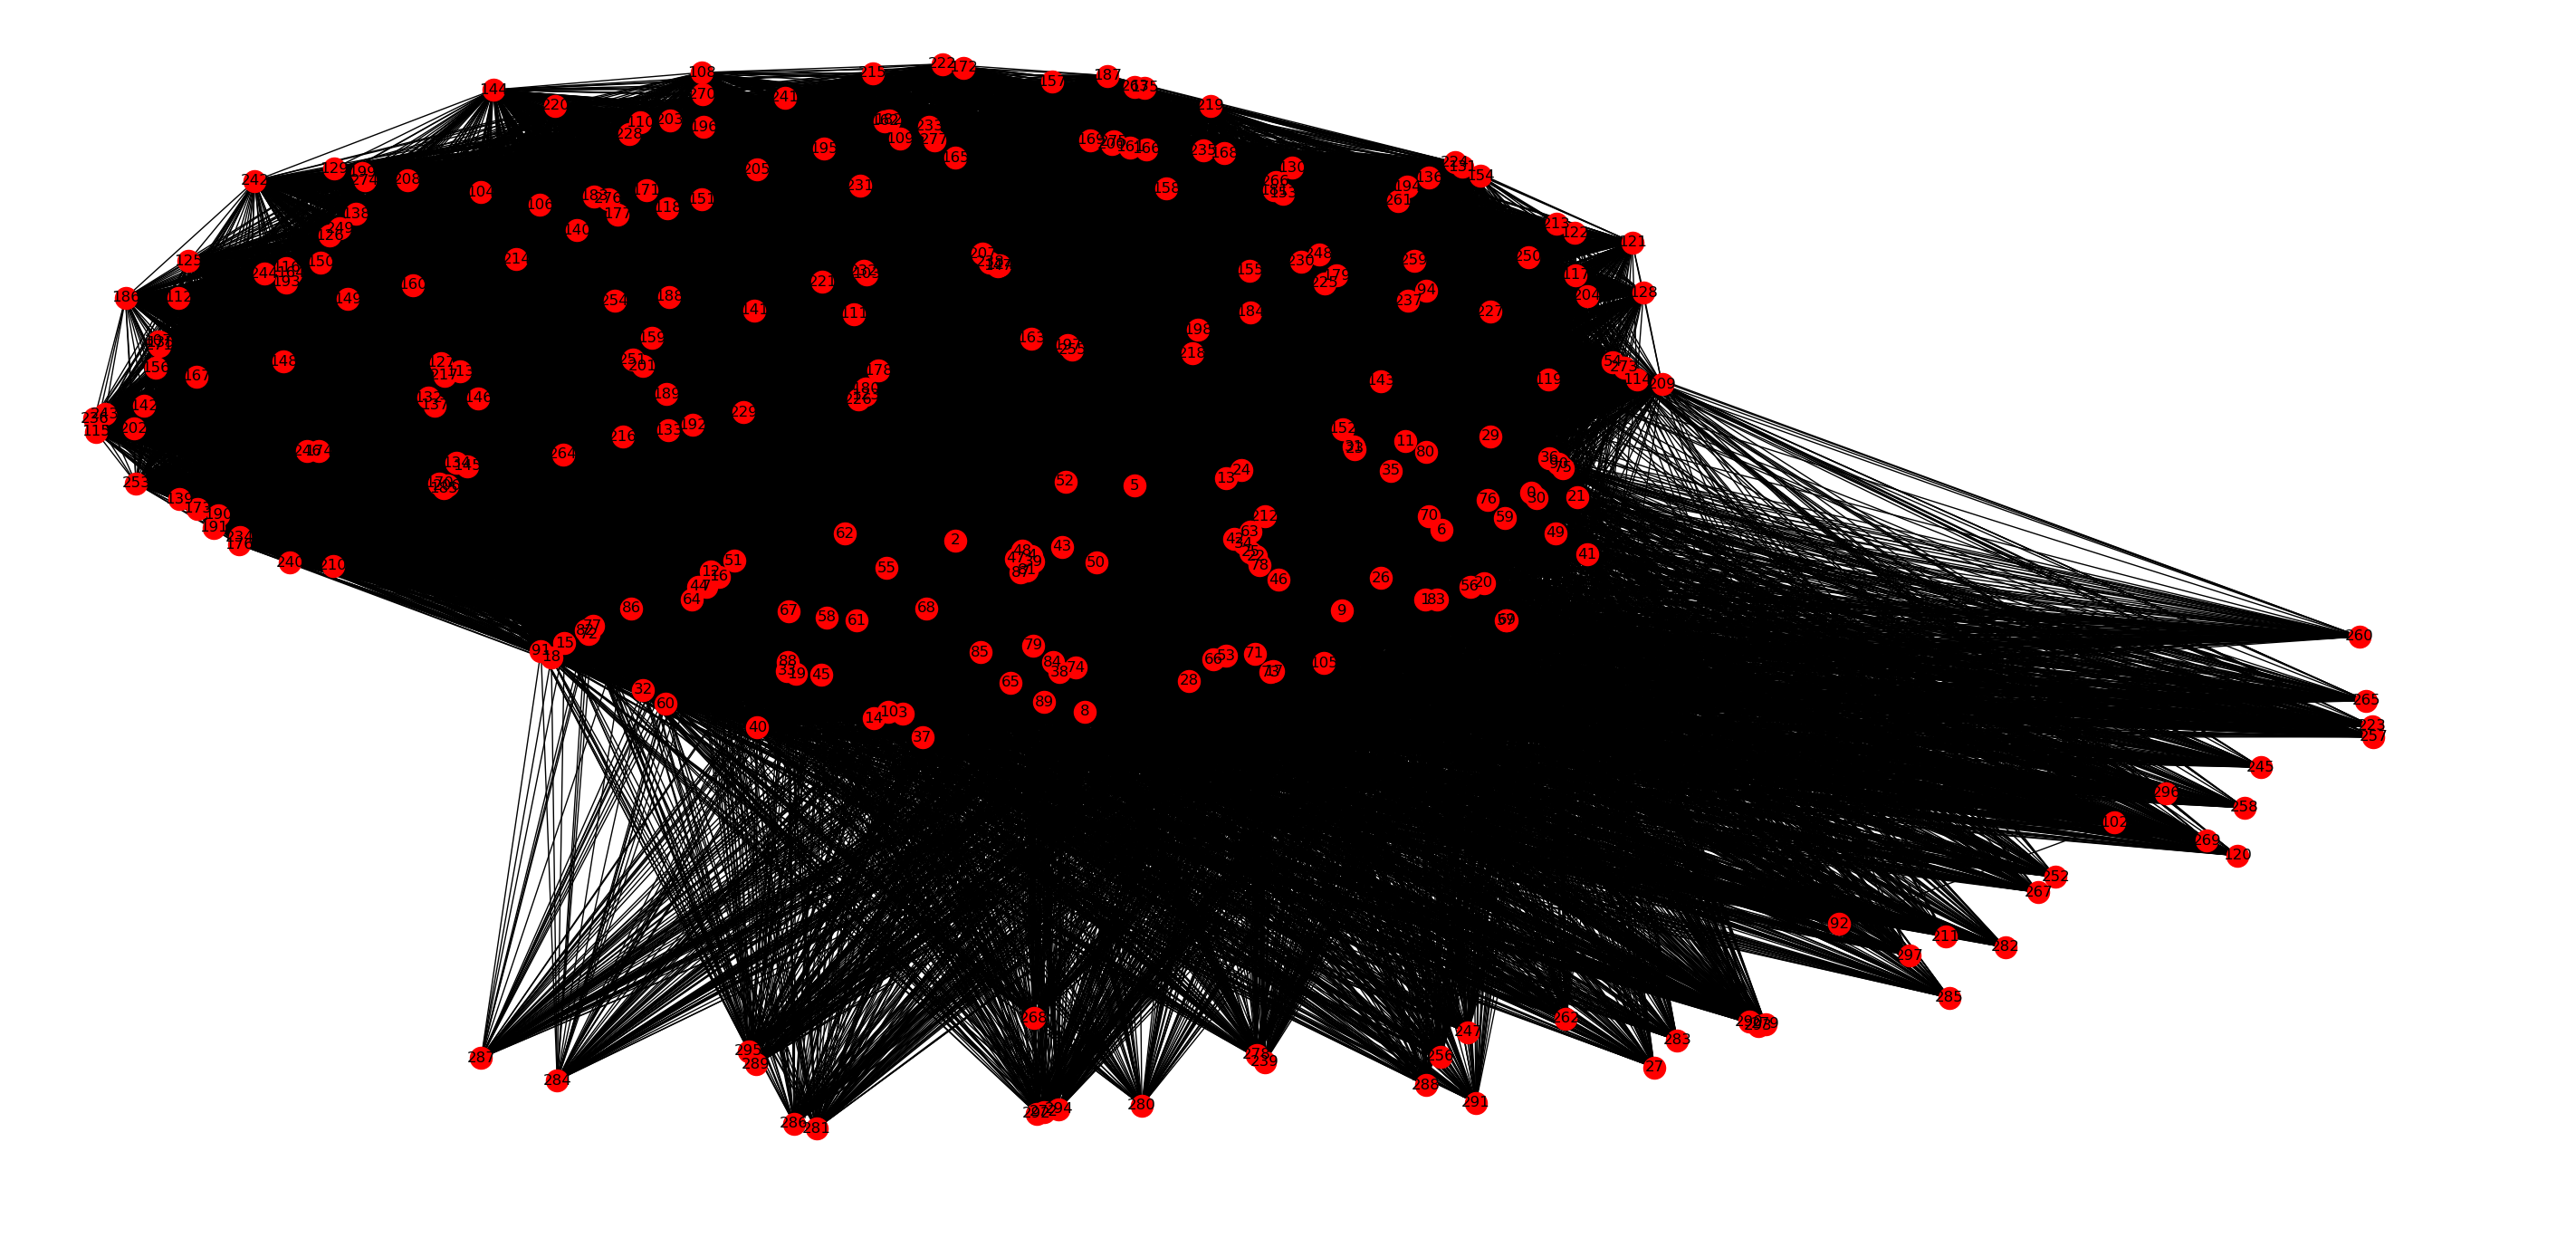
\includegraphics[width=1.0\linewidth]{SchemaSummarization/img/YelpCovMat.png}
\caption{Coveriance Cloud for the full Yelp dataset.}
\label{fig:cloud}
\end{figure}

\tinysection{Covariance Clouds}
Our second visual representation, also like schema summaries, uses correlations and anti-correlations to communicate subschemas of interest.
To generate a covariance cloud, we create a covariance matrix from the source schemas, using the appearance of each attribute as a variable.
Based on a user-controllable threshold, we then construct a graph from the covariance matrix with every attribute as one node, and every covariance exceeding the threshold as an edge.
The graph is then displayed to the user as a cloud using standard force-based layout techniques (e.g., those used by GraphViz~\cite{DBLP:conf/gd/EllsonGKNW00}).  
%\todo{Will: Add figure here}
Cliques in the graph represent commonly co-occurring subschemas that might form segments of interest.  
This includes every conjunctive group identified in the schema summary.
However, unlike the schema summary, this visual representation more effectively captures subschemas with attributes in common.

\tinysection{KNN-PCA Clouds}
While the first visualizaton works on simple schemas, we found that on more complex \json data like Twitter streams~\cite{twitterdecahose}, or the Yelp open dataset~\cite{yelpdata} there were too many inter-attribute relationships, and the resulting visualizatons were noisy.
An approach we settled on is a mixture of Principle Component Analysis (PCA) and K Nearest Neighbor clustering (KNN). 
As before, we treat each source schema as a feature vector with each attribute representing one feature. 
We then use PCA to plot our source schemas in two-dimensions.
The resulting visualization illustrates relationships between source schemas, with greater distances in the visualization representing (approximately) more differences between the schemas.
Hence, clustered groupings of schemas represent potentially interesting sub-schemas.

A key limitation with this visualization is that for more complex datasets the somewhat arbitrary choice of 2 dimensions can be too low.
Conversely adding more dimensions directly through PCA makes the visualization more complicated and hard to follow.
To mitigate these limitations, we use K-Nearest Neighbors (KNN) to colorize the PCA Cloud.
In addition to using PCA, we do KNN clustering on the schemas using a user-provided K (number of clusters).  
Each cluster identified by PCA is assigned a different color.
Combined, these two algorithms to provide users an initial insight into the potential correlations that exist in their dataset.


\begin{figure}
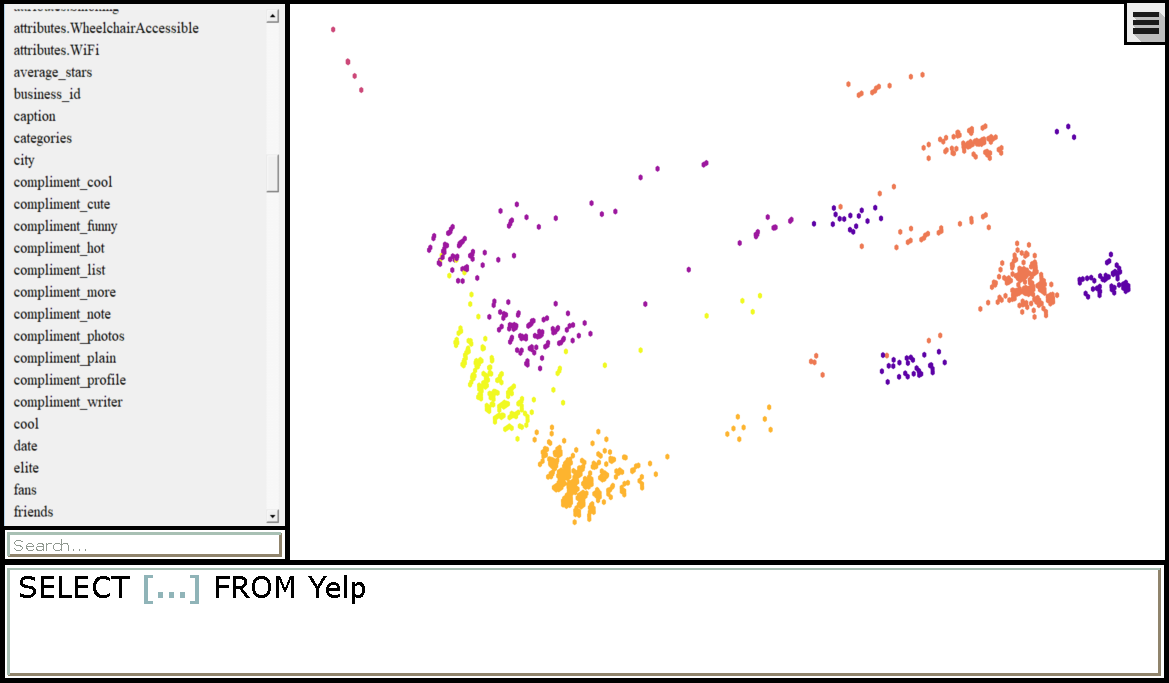
\includegraphics[trim={50mm 25mm 5mm 10mm},clip,width=1.0\linewidth]{SchemaSummarization/img/YelpUI.pdf}
\caption{KNN-PCA cloud with K=6 on the Yelp dataset.}
\label{fig:yelp}
\end{figure}

\begin{example}
Figures~\ref{fig:ui} and \ref{fig:yelp} show an example of the resulting view on Twitter and Yelp data.
Note the much tighter clustering of attributes in the Twitter data: each cluster represents one particular, common type of tweet.
Conversely, the Yelp schema includes a nested collection with, for example, hourly checkins at the business.  
The presence (or absence) of these terminal paths is more variable, and the resulting PCA cloud follows more of a gradient.
\end{example}

These graphs may not initially be intuitive to interpret, but they provide abstract bearings that map directly to phenomenon’s that exist in the data. In lieu of a formal user study, we postulate that the information gained from each algorithm independently will benefit the exploration process that is agnostic to labeled information. This is in contrast to other tools~\cite{Smith:2006:FSS:1187627.1187785}, that largely utilize naming cues and attribute nesting to meet user needs.

\subsection{Schema Exploration}

Now that we have shown the user potentially interesting subschemas, our next task is to help them to (1) narrow down on actually interesting subschemas, and (2) use those schemas to drill down to a segment of the schema data.
For the first step, it is critical that the user develop a good intuition for what the visual representations encode.
One way to accomplish this is to establish a bi-directional mapping between \systemnametwo's two data panes.

To map from visual survey to schema summary, we provide users with a lasso tool.
As illustrated in Figure~\ref{fig:ui}, users can select regions of the KNN-PCA Cloud and the corresponding schemas within that region.  Doing so identifies the maximal subschema contained in all subschemas and regenerates the schema summary pane based only on the segment containing the maximal subschema.  
The maximal subschema itself is also highlighted in the schema summary pane.
On the Covariance cloud, the lasso tool behaves similarly, selecting attributes explicitly rather than a maximal subschema.

The reverse mapping is achieved using highlighting, as illustrated in Figure~\ref{fig:yelpH}.
Users can select one or more attributes (or groupings) in the schema summary pane, and the KNN-PCA Cloud (resp., Covariance Cloud) is modified to highlight schemas in the corresponding segment (resp., to highlight the attributes).
In conjunction with their prior knowledge of their tasks and ideal use cases, we use this approach to perform the initial schema segmentation.

% What patterns immerge and how do we present them
In either case, after selecting a set of attributes or schemas, the analyst may choose to drill down into the selected segment, regenerating both views for the now restricted collection of schemas.
% An analyst may then futher collapse this tree, to produce a view that they can query. Segmentation provides the ability to display tight groups of highly correlated attributes, instead of a large spanning tree that is impossible for a human to process by hand.



% %Attribute co-occurrence can be caused by the presence of an underlying sub-schema and if many co-occur this indicates the presence of a secondary schema, similar to an entity. 
% Segmenting our data first into these entities and then summarizing them, allows us to present the user with features that describe each entity in smaller doses. 
% Additionally, the existence of these entities is derived from insertion methods, and by extension data collection methods, which correspond to natural groupings of attributes that a user expects.


\begin{figure}
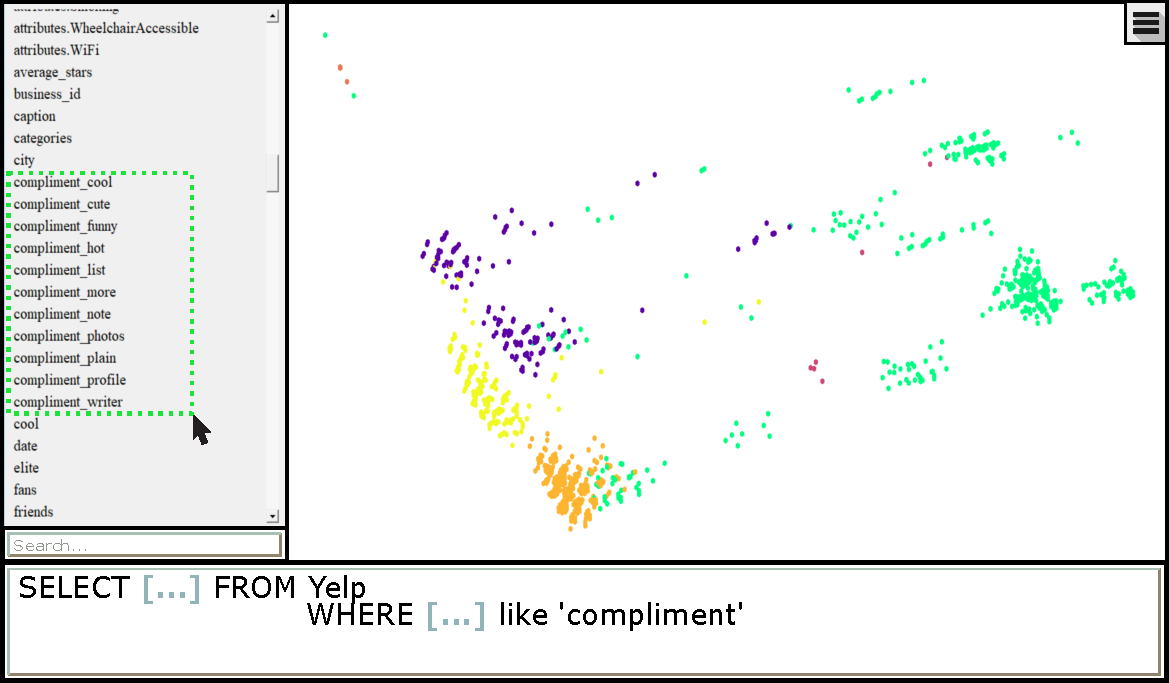
\includegraphics[width=1.0\linewidth]{SchemaSummarization/img/YelpUIH.pdf}
\caption{Points containing user selected attributes are highlighted green.}
\label{fig:yelpH}
\end{figure}


%\begin{itemize}
%\item cov matrix clique issues
%\item knn limitations
%\item PCA limitations and benefits
%\item goal is to first reduce the 
%\end{itemize}

%Through our user interface groups of attributes may be highlighted, this then feeds back into our PCA plot to highlight the points that these attributes are present in. 
%If this group of attributes has high co-occurrence, then they are likely to appear grouped and ideally leads the user to other attributes that also co-occur and are of significance.

\subsection{An Iterative Approach}
At any time in our exploration pipeline analysts may stop where they are, take the knowledge they gained about their dataset, and restart the process from the beginning. 
Through exploring the Twitter dataset we found retweets and quoted tweets to have a high correlation, with this knowledge we can then start back at the beginning and depending on whether our task allows us to merge these attributes, we can then choose a more appropriate K value for KNN. 
In addition, attributes that have no relationship to core attributes, such as a users profile\_image\_url being present, can easily be pruned to compress our summary output. 
By incrementally learning about their dataset, an analyst can converge on the views required for their tasks.


%Will: How does the data get summarized for user consumption. 
%Some UI sketches/screenshots would be appropriate.
%\begin{itemize}
%\item The schema is presented to the user
%\item The user is then shown a 2-dimensional representation of their data using PCA
%\item Iteratively use a generic clustering algorithm to help detect clusters and relationships in their data
%\item Select a subregion of the map to expore relaitonships that exist and what each group represents
%\item |eigenVector| x norm($\sum\nolimits $multiplicity x featureVector), this results in a score for each column that is based on occurance and variation
%\item the higher this score, the more 'representative' of the cluster this feature is
%\item Iterate through this process to determine what the defining characteristics of each group is, and how it relates to other groups
%\end{itemize}




% \section{Iteration}
% \label{sec:iteration}
% 

What facilities do users have for probing for more information, refining the current view, and/or marking the current view as sufficient.

% \section{Experiments}
% \label{sec:experiments}
% 

Time and space permitting...

\section{Related Work}
\label{sec:related}
% -*- root: ../cnf-json.tex -*-
 \tinysection{Schema Extraction}
Schema extraction for \json, as well as for other self-describing data models like XML has seen active interest from a number of sources. 
An early effort to summarize self-describing \emph{hierarchical} data can be found in the LORE system's DataGuides~\cite{DBLP:conf/vldb/GoldmanW97}.
DataGuides view schemas begin with a forest of tree-shaped schemas and progressively merge schemas, deriving a compact encoding of the forest as a DAG.
Although initially designed for XML data, similar ideas have been more recently applied for \json data as well~\cite{DBLP:conf/cidr/LiuG15,DBLP:conf/sigmod/LiuHMLC16}.
Key challenges in this space involve simply extracting schemas from large, multi-terabyte collections of \json data~\cite{DBLP:conf/edbt/BaaziziLCGS17}, as well as managing ambiguity in the set of possible factorizations of a schema~\cite{DBLP:conf/dbpl/BaaziziCGS17,spoth:2017:cidr:adaptive}.
The approach taken by Baazizi et. al.~\cite{DBLP:conf/edbt/BaaziziLCGS17} in particular adopts a type unification model similar to ours, but lacks the conjunctive operator of our type-system.
For non-hierarchical data, interactive tools like Wrangler~\cite{DBLP:conf/chi/KandelPHH11} provide an interactive frameworks for regularizing schemas.

\tinysection{Physical Layout}
While schemas play a role in the interpretability of a \json data set, they can also help improve the performance of \json queries.  
One approach relies on inverted indexes~\cite{DBLP:conf/cidr/LiuG15} to quickly identify records that make use of sparse paths in the schema.
Another approach is to normalize schema elements~\cite{DBLP:conf/sigmod/DiScalaA16}.  Although the resulting schema may not always be interpretable, this approach can result in substantial space savings.

\tinysection{Information Retrieval}
From a more general perspective, the schema extraction problem which aims at making large datasets tractable for interactive exploration, is an instance of \textit{categorization} problem that has been repeatedly studied in the literature.
More precisely, attributes (metadata) of the datasets can be grouped into a hierarchy of "facets" (i.e., categories)~\cite{Smith:2006:FSS:1187627.1187785} where the child-level facets are conditioned on the presence of the parent one.
In our approach, we adopt the hierachical data visualization and focus more on the algorithmic essence of the problem: How to (1) balance between the preciseness and conciseness of the visualization and (2) respond to users' data exploration requests in a scalable way.

\section{Future Work}
\label{sec:future}
% !TEX root = ../cnf-json.tex
One challenge that we will need to address in \systemnametwo is coping with nested collections.  
At the moment, the user can manually merge collections of attributes that correspond to disjoint entites.
However, we would like to automate this process.
One observation is that a typical collection like an array has a schema with the general structure:
$$(P_1 \vee P_1P_2 \vee P_1P_2P_3 \vee \ldots)\;=\;(P_1 \wedge (\emptyset \vee P_2 \wedge (\emptyset \vee P_3 \wedge (\ldots)) ))$$
The version of this expression on the right hand side is notable as its closure over the semiring $\tuple{\big\{\{\mathbf P\}\big\}, \vee, \wedge, \emptyset, \big\{\{\}\big\}}$ would indicate that the semiring is ``quasiregular'' or ``closed'', an algebraic structure best associated with the Kleene star.
Hence, we plan to explore the use of the Kleene star to encode nested collections in our algebra.
A key challenge in doing so is detecting opportunities for incorporating it into a summary, a more challenging form of the factorization problem.

A further step to increase the capabilities of \systemnametwo is to incorporate type information in the summarization. 
This adds an extra layer of information an analyst can extract from our system, as well as the ability to identify and correct schema errors. 
As a long term goal we will provide capabilities for linking views, for example by defining functional dependencies.
The goal is to create full entity relationship diagrams. 
In particular, one interesting way to identify potential relationships that exist between entities is by leveraging the overlap between segments.
